%!TEX root = ../report.tex

\begin{document}
    \chapter{State of the Art}
    In this chapter, we will discuss about the 3D LiDAR datasets available and made an attempt to classify them based on type of acquisition.
    Also we will discuss about the 3D semantic segmentation models, uncertainty estimation methods and OOD methods available.
    \section{3D LiDAR Datasets}
    %Since the advent of AlexNet \cite{alexnet}, deeplearning has been in the rise. 
    %Deep convolutional neural networks are the desired option for image analysis tasks such as classification, detection and segmentation.
    %These deep convolutional networks are successful especially because of two reasons. 
    %First is the architectures and their paralellisation, allowing them to train millions of images on a GPU.
    %Second reason is the development of huge public benchmark datasets such as Imagenet \cite{imagenet}, Pascal VOC \cite{pascalvoc} and COCO \cite{coco} datasets
    %Although deep convolutional networks are huge success in image analysis tasks, they perform poorly on 3D point cloud data.
    LiDAR is one of the central component in the sensor suite for SLAM system in robotic applications \cite{thrun2006stanley}, \cite{patz2008practical}, \cite{hess20162dSLAM} and autonomous driving \cite{li2016vehicle}.
    3D LiDAR data is preferred because, it can provide the exact replica of 3D geometry of the real world represented in the form of 3D point clouds.
    Because of these rich features and widespread use of LiDAR sensors, tasks such as 3D object detection \cite{zhou2018voxelnet}, \cite{PIXOR} and 3D semantic segmentation \cite{qi2017pointnet++}, \cite{3Dmininet} are becoming more predominant area for research.
    
    In this section, we will discuss about the available 3D LiDAR datasets for 3D semantic segmentation task and classify the datasets based on acquisition methods as in \cite{survey3d}.
    \cite{survey3d} classifies the available public datasets into three classes based on the data acquisition process.
    They are \textit{Sequential}, \textit{Static} and \textit{Synthetic} datasets.
    The data for sequential datasets are collected as frame sequences where mechanical LiDAR is mounted on top of a autonomous driivng platform as in Figure \ref{fig:seq_data_lyft}.
    \begin{figure}[h!]
        \centering
        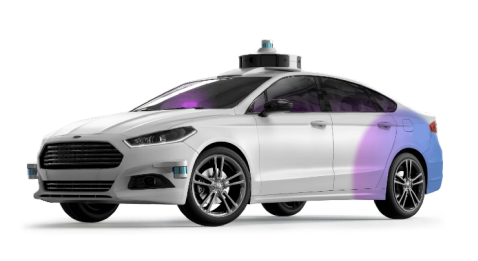
\includegraphics[scale=0.25]{images/sequential_lyft.png}
        \caption{Sequential mounted LiDAR for data collection of Lyft L5 dataset. Image from \cite{Lyftl5}}
        \label{fig:seq_data_lyft}
    \end{figure}
    Most of the popular autonomous driving datasets are of sequential type, but these kind of datasets comes with a drawback of sparse points than other datasets.
    
    Static datasets consists of data collected from a stationary view point by a terrestrial laser scanner.
    These kind of datasets capture the static information of the realworld whereas the sequential datasets capture the dynamic movements of the surrounding objects.
    Static datasets find their way in applications such as the urban planning, augmented reality and robotics. 
    Figure \ref{fig:tls} depcits a terrestrial laser scanner used to capture point cloud of an industrial environment.
    \begin{figure}[h!]
        \centering
        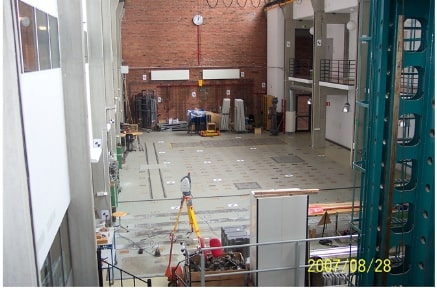
\includegraphics[scale=0.75]{images/TLS.jpg}
        \caption{Terrestrial laser scanner in an industrial environment with the laser scanner mounted on a yellow tripod in the left corner of the floor. Image taken from \cite{tls}}
        \label{fig:tls}
    \end{figure}
    An advantage with the static datasets, are they can produce highly dense point clouds leading to rich 3D geometric representations.
    
    Last type of 3D LiDAR datasets are synthetic datasets. 
    As the name suggests these datasets are generated from the computer simulation. 
    Figure \ref{fig:synthetic} depcits a simulated point cloud in a synthtic dataset called SynthCity.
    Eventhough synthetic datasets can be generated in large scale with cheap cost, they lack the accuracy in detail when compared to the point clouds generated from real world.
    \begin{figure}[h!]
        \centering
        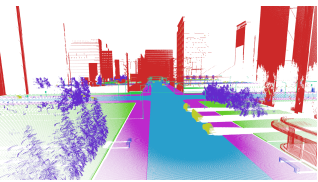
\includegraphics[scale=0.5]{images/synthcity.png}
        \caption{Illustration of a scene in synthetic dataset called SynthCity. Image taken from \cite{griffiths2019synthcity}}
        \label{fig:synthetic}
    \end{figure}
    
    The datasets belonging to the each acquisition type are summed up in  Table \ref{table:3d_lidar_datasets_table}.
    Most of the datasets from the Table \ref{table:3d_lidar_datasets_table} are taken from \cite{survey3d} and also as a part of this study, additional new datasets were added to the list.
    The newly added datasets include DALES \cite{varney2020dales}, ScanObjectNN \cite{scanobejctnn} in static acquisition mode and AIO Drive \cite{Weng2020_AIODrive}, Toronto3D \cite{tan2020toronto3d} are additions in the sequential mode.
    \cite{survey3d} also classifies GTAV \textcolor{red}{\textbf{cite}} dataset as synthetic 3D LiDAR but the corresponding paper doesn't report any LiDAR dataset and proposed only 2D dataset for segmentation.
    The limited number of datasets in 3D LiDAR allowed us to study the characteristics of each individual datasets such as each class, data distribution and features of each point in point cloud. 
    It is summarized in Table \textcolor{red}{\textbf{ref}} in Appendix \textcolor{red}{\textbf{chapter number}}
    %%\section{TODO}
    %%\begin{itemize}
    %%     \item[$\bullet$] Explain the table
    %%    \item[$\bullet$] Discuss why SemanticKITTI and Semantic3D are of our interest     
    %%\end{itemize}
    
    \begin{table}[h!]
        %\centering
        \begin{tabular}{c|c|c|c|c|c}%|c}
            \hline
            % acquisition type, dataset, frames, #points, classes, I/O, year
            acquisition mode & dataset & frames & points (in million) & classes & scene type \\  % & pub. year \\
            \hline
            \multirow{7}{*}{static} & Oakland\cite{oakland} & 17 & 1.6 &  44 & outdoor \\ % & 2009 \\ 
                                    & Paris-lille-3D\cite{roynard2018paris} & 3 & 143 & 50 & outdoor \\ % & 2018 \\
                                    & Paris-rue-Madame\cite{paris_rue_madame} & 2 & 20 & 17 & outdoor \\ %& 2014 \\
                                    & S3DIS\cite{Armeni_2016_CVPR_S3DIS} & 5 & 215 & 12 & indoor \\ %& 2016 \\
                                    & ScanObjectNN\cite{scanobejctnn} & - & - & 15 & indoor \\ %& 2019 \\
                                    & Semantic3D\cite{hackel2017semantic3d} & 30 & 4009 & 8 & outdoor \\ %& 2017 \\
                                    & TerraMobilita/IQmulus\cite{TerraMobilita} & 10 & 12 & 15 & outdoor\\ % & 2015 \\
                                    & TUM City Campus\cite{gehrung2017approach_tum_campus} & 631 & 41 & 8 & outdoor\\ % & 2016 \\
                                    & DALES\cite{varney2020dales} & 40 (tiles) & 492 & 8 & outdoor\\ % & 2021\\
            \hline
            \multirow{7}{*}{sequential} & A2D2\cite{geyer2020a2d2} & 41277 & 1238 & 38 & outdoor\\ % & 2020\\
                                        & AIO Drive\cite{Weng2020_AIODrive} & 100& - & 23 & outdoor\\ % & 2020\\
                                        & KITTI-360\cite{Xie_2016_CVPR_KITTI_360} & 100K & 18000 & 19 & outdoor\\ %& 2020\\
                                        & nuScenes-lidarseg\cite{caesar2020nuscenes} & 40000 & 1400 & 32& outdoor\\ % & 2020\\
                                        & PandaSet\cite{PandaSet} & 16000 & 1844 & 37 & outdoor \\ %& 2020\\
                                        & SemanticKITTI\cite{Behley_2019_ICCV} & 43552 & 4549 & 28 & outdoor \\ %& 2019\\
                                        & SemanticPOSS\cite{pan2020semanticposs} & 2988 & 216 & 14 & outdoor \\ %& 2020\\
                                        & Sydney Urban\cite{de2013unsupervised} & 631 & - & 26 & outdoor\\ % & 2013\\
                                        & Toronto-3D\cite{tan2020toronto3d} & 4 & 78.3& 8& outdoor\\ % & 2020\\
    
            \hline
            \multirow{1}{*}{synthetic}  & SynthCity\cite{griffiths2019synthcity} & 75000 & 367.9 & 9 & outdoor \\ %& 2019\\
            \hline
        \end{tabular}
        \caption{3D LiDAR datasets classified based on the acquisition type. Table updated from \cite{survey3d}}
        \label{table:3d_lidar_datasets_table}
    \end{table}
    
    From the available datasets, we chose Semantic3D dataset as in-distribution (ID) training dataset. 
    S3DIS is chosen as out-of-distribution (OOD) dataset as S3DIS is much different from Semantic3D.
    Detailed disussion on datasets were done in Chapter \textcolor{red}{cite here}.

    \section{3D semantic segmentation models}

In this section, we will discuss about the methods available for 3D semantic segmentation.
The discussion include a breif peek into traditional 3D semantic segmentation methods and study of deep learning based 3D point cloud segmentation.

Traditional methods involve a complex features extraction and pass these features to a classficiation algorithm such as Support Vector Machines or Random Forests to classify each point the point cloud.
Various authors developed variety of methods to extract the features from the input point cloud.
Some of these methods include segmentation from edge information \cite{bhanu1986range}, construction of complex graph pyramids \cite{koster}.
3D Hough transforms as in \cite{vosselman20013d} and application of RANSAC \cite{schnabel2007efficient} and \cite{tarsha2007hough}.
These traditional methods are now outdated as DNNs proved to better at feature extraction.

\subsection{Deep learning based 3D semantic segmentation}
Deep learning based models are efficient at segmentation and can be divided into three types.
Initial type include the point based models where the model directly feeds on the 3D point cloud.
Then the other type include projection based models where the model takes in a projected points into 2D image either a range image or bird's eye view.
Final type of models include the use of graph neural networks.
Point based models mostly utilize fully connected layer or convolutional layers. 
Where as the projection based models utilize existing 2D semantic segmentation archiecture.
The detailed summary of each model belonging to these two categories are depicted in Table \ref{tab:model_relatedwork} along with number of parameters.
Finally, graph neural networks are out of the scope for this project and will not be disucssed further.
\begin{longtable}{|p{0.15\linewidth} | p{0.59\linewidth}| p{0.06\linewidth} |p{0.09\linewidth}|}
    %\centering
    %\begin{tabular}{|p{0.15\linewidth} | p{0.6\linewidth}| p{0.06\linewidth} |p{0.08\linewidth}|}
        \hline
        \textbf{Method} & \textbf{Summary} & \textbf{Type} & \textbf{\#Params} \\
        \hline 
        PointNet\cite{Qi_2017_CVPR_pointnet} &
        PointNet works on raw point cloud and acheives permutation invariance of point cloud by using maxpooling as symmetric function.
        Transformation invariance of point cloud is acheived by generating a transformation matrx generated by Spatial Transformer Network.
        gloabl features are extracted by maxpooling layer and fed into segmentation head for 3D segmentation.
        & Point & 3M \\
        \hline
        PointNet++\cite{qi2017pointnet++} &
        PointNet doesnt capture local structures becuase of only global features extraction.
        So PointNet++ applies PointNet recursively on portions of input point cloud to extract featuers and these are grouped to form high level features.
        & Point & 6M \\
        \hline
        TangentConv\cite{Tatarchenko_2018_CVPR_tangconv} &
        Proposes tangent convolutions which are simialr to normal convolution but an additional multiplication of gaussian kernel.
        The architecture is encoder-decoder style with fully convolutional network consisting of tangent convolutions.
        & Point & 0.4M\\
        \hline
        SPLATNet\cite{Su_2018_CVPR_splatnet} &
        This model uses Bilateral Convolutional Layers(BCL) to project data onto low dimensional lattice.
        These lattices from BCL are then convolved and reprojected back to the point cloud.
        USe of BCL allows the projection 2D semantic labels to label the 3D point cloud.
        & Point & 0.8M \\
        \hline
        SqueezeSeg\cite{Sequeseseg_2018} &
        Projects the data onto 2D spherical coordinates and segmented using SqueezeNet.
        The segmented 2D image is reprojected back to 3d using Recurrent Conditional Random Fields.
        & Project & 1M \\
        \hline
        SqueezesegV2\cite{SqueezeSegv2} &
        Extension over SqueezeSeg by using Context Aggregation Module (CAM) before encoder to minimize the effects of missing points on convolutional filters of SqueezeSeg.
        Proposed novel focal loss instead of weighted cross entropy to better represent the dataset class imbalance.
        & Project & 1M \\
        \hline
        SqueezesegV3\cite{xu2020squeezesegv3} &
        Spherical proejction based model which uses Spatially Adaptive Convolutions to change filters according to the differnt locations in the input image.
        The architecture is similar to RangeNet with cross entropy loss calculated at each layer.
        & Project & 0.92M \\
        \hline
        %SPGraph\cite{SPGraph} & & Point & 0.25M\\
        %\hline
        LatticeNet\cite{rosu2019latticenet}\footnote{LatticeNet has no code to calculate number of parameters} &
        The input point cloud is projected onto d-dimensional sparse lattice and reprojection is learnt form the data by using novel proposed DeformSlice module.
        The architecture is similar to U-Net with lattice projeciton at encoder and DeformSlice at end of decoder module.
        & Point & - \\
        \hline
        RangeNet-21\cite{Milioto2019} & 
        Spherical projection based model with encoder-decoder style architecture with encoder being DarkNet21.
        Introduced a better evaluation metric called borderIoU for occlusions.
        & Project & 25M \\
        \hline
        RangeNet-53\cite{Milioto2019}  & 
        Architecturally similar to RangeNet-21, the only change is encoder which is DarkNet53.
        No postprocessing is applied for occlusions or nonprojected points.
        & Project & 50M \\
        \hline
        RangeNet-53++\cite{Milioto2019} &
        RangeNet-53++ architecture is same as RangeNet-53 but a post processing 
        method of kNN is applied on output to label the occluded points or nonprojected points after reprojection from segmented 2D spherical image to 3D points.
        & Project & 50M \\
        \hline
        RandLA-Net\cite{Hu_2020_CVPR_Randla} & 
        Random points from input point cloud are sampled and fed into local feature aggregation (LFA) module for feature extraction.
        These fetures are weighted and selected based on the attention score. 
        Encoder-decoder style architecture with stacks of LFA as encoder and decoder is transponse convolutions for upsampling with MLP followed by fully connected layers for segmentation.
        & Point & 0.95M \\
        \hline 
        3DMiniNet\cite{3Dmininet} &
        This model works on spherical projection of 3D point cloud which is fed into projection learning module to learn local and global features.
        These learnt features are fed into MiniNetV2 which is a fully connected neural network for segmentation of spherical image.
        This 2D image is reprojected back into 3D point cloud using kNN search as in RangeNet53++.
        & Project & 4M \\
        \hline
        SalsaNet\cite{salsanet2020} & Encoder-decoder style architecture with Bird-Eye-View projection as input and encoder consisting of ResNet blocks and decoder with transpose convolutions.
        Unlabelled points in LiDAR are auto labelled from corresponding images. Claims SalsaNet is projection agnostic.
        & Project & 6.6M \\
        \hline
        SalsaNext\cite{SalsaNext_2020} & 
        Similar architecture to SalsaNet, proposed a new context module replacing ResNet module in encoder and pixel shuffle instead of transposed convolutions in decoder.
        Proposed Lovasz-Softmax loss in combination with weighted cross-entropy loss.
        This is the first model best of our knowledge to study epistemic and aleatoric uncertainty by modelling SalsaNext as Bayesian Neural Network.
        & Project & 6.7M \\
        \hline
        PolarNet\cite{polarnet} &
        It is a projection based model, instead of spherical or bird's eye view projection in cartesian coordinate system, this model projects the data into bird's eye view projection on to a grid of polar coordinate system.
        This grid is a fixed size representation and features are extracted are for each grid cell.
        & Project & 14M \\
        \hline
        KPRNet\cite{kochanov2020kprnet} &
        Projects the data into 2D spherical image and 2D CNN encoder-decoder architecture is applied.
        Encoder consists of ResNeXt-101 and decoder is similar to DeepLab with depthwise seperable convolutions.
        Backprojection to 3D is made using KPConv similar to KNN in RangeNet-53++.
        & Project & 243M \\
        \hline
        SPVNAS\cite{spvnas} &
        Proposes Sparse Point-Voxel Convolutions (SPVConv) aimed to improve performance over small objects such as pedestrains, cyclistis.
        SPVConv voxelizes point cloud and apply sparse convolution and then devoxelizes the voxel to point cloud.
        This is the first 3D semantic segmentation model to utlize Neural Architecture Search (NAS).
        & Point & 2.6M \\
        \hline
        Cylinder3D\cite{zhu2020cylindrical}\footnote{Cylinder3D uses Sparse Convolutions which are not supported in Ubuntu-20 at the time of study.} &
        Converts 3D cartesian coordinates to 3D cylinder coordinates then voxelizes and fed into Asymmetric Residual Block to extarct these cuboid features.
        These features are applied to 3D U-Net for segmentation.
        & Project & - \\
        \hline
        %(AF)2-S3Net\cite{af2s3net} & & Point & - \\
        %\hline
        \caption{Summary of various point and projection based 3D semantic segmentation models. In Type column point represent point based model and project represents projection based model.}
        \label{tab:model_relatedwork}
    %\end{tabular}
\end{longtable}

    We chose RandLA-Net as the model because of its ability to extract complex structures and lower parameters.
    Detailed reasons and explanation about RandLA-Net is discussed in Section \textcolor{red}{cite here}.

    \section{Uncertainty estimation methods}
    In this section we will discuss about existing methods to estimate uncertainty in deep neural networks.
    Here we divide the existing methods into ensemble methods, bayesian method and others.
    The methods discussed here mostly estimate epistemic uncertainty only test time augmentation and gaussian density models estimate aleatoric unceratinty.
    \subsection{Ensemble methods}
    Deep ensembles first proposed in  \cite{lakshminarayanan2016simple} are the most prominently used methods for the uncertainty estimation.
    They exploit the combinatory power of multiple models. Each input is fed into a model with multiple instances and the each instance of the model is initalized randomly.
    This leads to slightly different optimization for each of the instance of the model. The final output scores from each model are combined by simple averaging.
    Deep ensembles are known to improve overall performance of the model but comes with a cost of computational complexity and resource intensiveness.
    Another advantage of using deep ensembled are the lowest correaltion between the model instances as the training of the instances are done differently.
    This lower correlation figures lead to diverse prediction from each model instance.
    In detailed explantion about deep ensembles can be found in Chapter \textcolor{red}{cite} Section \textcolor{red}{cite}.

    Because of the higher computational complexity and resource intensiveness, multiple flavours of the deep ensembles are proposed such as deep sub-ensembles \textcolor{red}{cite} and masksembles \textcolor{red}{cite}.
    In deep sub-ensembles, the network is divided into two parts called trunk and head.
    The main idea here is to train multiple instances of the head with the same trunk. For example, a trunk can be feature extraction layers in a deep classification network and the head can be the classification layers.
    Since the major motivation of the subensembles is to improve the training speed the performance lacks minutely when compared to deep ensembles as it is a tradeoff between the computational time and quality of uncertainty.
    Masksembles proposed in \textcolor{red}{cite} are realtively new and are a combination of deep ensembles with MC-Dropout.
    Dropout proposed in \textcolor{red}{cite} includes dropping of random neurons where as here a predefined mask is stated for each layer and only those certain neurons are to be dropped everytime.

    Other methods include snapshot ensembles \textcolor{red}{cite} which iterates over the multiple local optima in the optimization landscape using cyclic learning rate. 
    The model parameters are saved at each of the local optima. 
    All of the other flavors of deep ensembles are proposed in order to reduce the effect on time but the memory requirements remain mostly the same except the subensembles.
    The other problem with snapshot ensembles are the optimization landscape in deep neural networks are poorly studied, so there one cannot say with certainty that model saved at two local minima are uncorrelated.
    There also exists neural ensemble search \textcolor{red}{cite} where the nerual archiecture search is applied over the ensembles.
    Instead of using various instances of the same model, authors in \textcolor{red}{cite above paper} use vaiours instances of various models in the archiecture search space.
    Finally, all the above discussed ensmeble models can be group under sampling based methods, because each image is passed to mulitple model instances.    

    \subsection{Bayesian methods}
    \section{Out-of-distribution (OOD) detection methods}
\end{document}
